%%%%%%%%%%%%%%%%%%%%%%%%%%%%%%%%%%%%%%%%%%%%%%%%%%%%%%%%%%%%%%%%%%%%%%%%%%%%%%%%%%
\begin{frame}[fragile]\frametitle{}

\begin{center}
{\Large Word2Vec: Theory}

{\tiny (Ref:The backpropagation algorithm for Word2Vec - Marginalia )}

\end{center}

\end{frame}

%%%%%%%%%%%%%%%%%%%%%%%%%%%%%%%%%%%%%%%%%%%%%%%%%%%%%%%%%%%%%%%%%%%%%%%%%%%%%%%%%%
\begin{frame}[fragile]\frametitle{What is Word2Vec?}
  \begin{itemize}
    \item The objective of word2vec is to find word embeddings, given a text corpus
	\item The size of the numerical vector can be decided by us.
	\item Two main architectures: Continuous Bag-of-Words (CBOW) and the Skip-gram model. 
	\item Simplest version of CBOW: a one-word window. Actual is typically 2 words on left, 2 words on right.
  \end{itemize}


\end{frame}

%%%%%%%%%%%%%%%%%%%%%%%%%%%%%%%%%%%%%%%%%%%%%%%%%%%%%%%%%%%%%%%%%%%%%%%%%%%%%%%%%%
\begin{frame}[fragile]\frametitle{Single Word CBOW}
  \begin{itemize}
    \item Input: the context is single word, $x$
	\item Output: the center word, $\hat{y}$
	\item Architecture: one input layer, one hidden layer and finally an output layer
	\item Activation for hidden layer : $a=1$
	\item Activation for output layer: $a=\mathbb{S}\textrm{oftmax}$
  \end{itemize}
  
\begin{center}
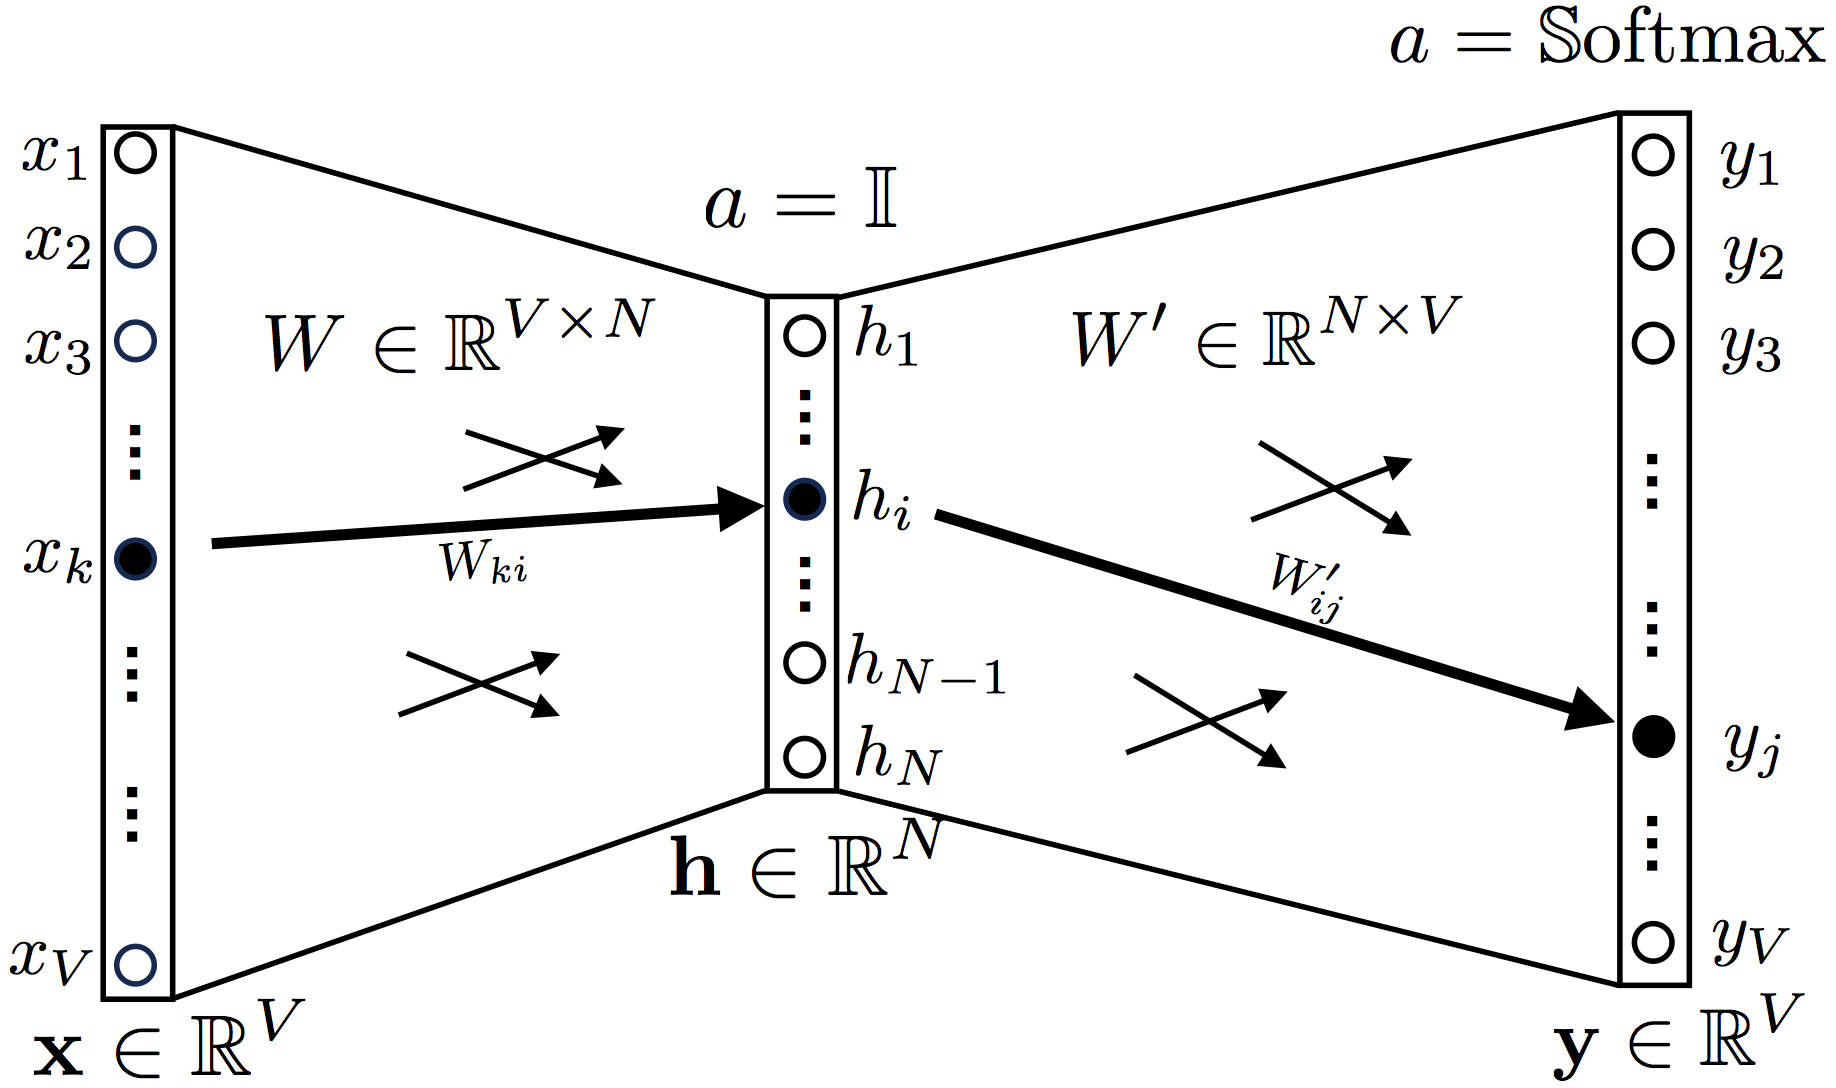
\includegraphics[width=0.6\linewidth,keepaspectratio]{w2v7}
\end{center}
\end{frame}

%%%%%%%%%%%%%%%%%%%%%%%%%%%%%%%%%%%%%%%%%%%%%%%%%%%%%%%%%%%%%%%%%%%%%%%%%%%%%%%%%%
\begin{frame}[fragile]\frametitle{Architecture}
  \begin{itemize}
    \item Input Layer:  one-hot encoded vector $x$ of dimension V, where V is the size of the vocabulary.
	\item Hidden Layer: dimension N, decided by us, typically 300.
	\item Output layer: again, one hot representation of output word, so is a vector of dimension V.
    \item Weights Matrix between input and hidden Layer: $W_{V \times N}$
    \item Weights Matrix between hidden and output Layer: $W'_{N \times V}$	
	\item The output vector $y$ should be close to $\hat{\textbf{y}}$
  \end{itemize}
  

\end{frame}

%%%%%%%%%%%%%%%%%%%%%%%%%%%%%%%%%%%%%%%%%%%%%%%%%%%%%%%%%%%%%%%%%%%%%%%%%%%%%%%%%%
\begin{frame}[fragile]\frametitle{Loss Function}
Calculate layers starting from left to right \ldots

\begin{eqnarray*}
\textbf{h} = & W^T\textbf{x} \hspace{7.0cm}  \\
\textbf{u}= & W'^T\textbf{h}=W'^TW^T\textbf{x} \hspace{4.6cm}  \\
\textbf{y}= & \ \ \mathbb{S}\textrm{oftmax}(\textbf{u})= \mathbb{S}\textrm{oftmax}(W'^TW^T\textbf{x})  \hspace{2cm}
\end{eqnarray*}

  \begin{itemize}
    \item Target (output) and Context (Input) word pairs: $w_t, w_c$
	\item Output word has $1$ at $j^{th}$ position, say.
	\item  Since the values in the softmax can be interpreted as conditional probabilities of the target word, given the context word 
$w_c$, we write the loss function as:
  \end{itemize}
  
\begin{equation*}
\mathcal{L} = -\log \mathbb{P}(w_t|w_c)=-\log y_{j^*}\ =-\log[\mathbb{S}\textrm{oftmax}(u_{j^*})]=-\log\left(\frac{\exp{u_{j^*}}}{\sum_i \exp{u_i}}\right),
\end{equation*}
\end{frame}

%%%%%%%%%%%%%%%%%%%%%%%%%%%%%%%%%%%%%%%%%%%%%%%%%%%%%%%%%%%%%%%%%%%%%%%%%%%%%%%%%%
\begin{frame}[fragile]\frametitle{Loss Function}
Finally, loss is:

\begin{equation}
% \bbox[lightblue,5px,border:2px solid red]{
\mathcal{L} = -u_{j^*} + \log \sum_i \exp{(u_i)}.
% }
\label{eq:loss}
\end{equation}

The loss function (Eqn \ref{eq:loss}) is the quantity we want to minimize, given our training example, i.e., we want to maximize the probability that our model predicts the target word, given our context word.

\end{frame}

%%%%%%%%%%%%%%%%%%%%%%%%%%%%%%%%%%%%%%%%%%%%%%%%%%%%%%%%%%%%%%%%%%%%%%%%%%%%%%%%%%
\begin{frame}[fragile]\frametitle{The backpropagation algorithm for the CBOW model}
  \begin{itemize}
    \item We want to find the values of $W$ and $W'$ that minimize the loss (Eqn \ref{eq:loss})
	\item Optimization problem is usually tackled using gradient descent
	\item To update the Weight matrices we need to find the derivatives  $\partial \mathcal{L}/\partial{W}$ and $\partial \mathcal{L}/\partial{W’}$
	\item The derivatives then simply follow from the chain rule for multivariate functions
	



  \end{itemize}

	\begin{equation}
\frac{\partial\mathcal{L}}{\partial W'_{ij}} = \sum_{k=1}^V\frac{\partial\mathcal{L}}{\partial u_k}\frac{\partial u_k}{\partial W'_{ij}}
\label{eq:dLdWp}
\end{equation}

and

\begin{equation}
\frac{\partial\mathcal{L}}{\partial W_{ij}} = \sum_{k=1}^V\frac{\partial\mathcal{L}}{\partial u_k}\frac{\partial u_k}{\partial W_{ij}}\ .
\label{eq:dLdW}
\end{equation}


\end{frame}


%%%%%%%%%%%%%%%%%%%%%%%%%%%%%%%%%%%%%%%%%%%%%%%%%%%%%%%%%%%%%%%%%%%%%%%%%%%%%%%%%%
\begin{frame}[fragile]\frametitle{The backpropagation algorithm for the CBOW model}
The weight $W’_{ij}$ which is an element of the matrix $W'$ and connects a node 
$i$ of the hidden layer to a node $j$ of the output layer, 
only affects the output score $u_j$ (and also $y_i$)

\begin{center}
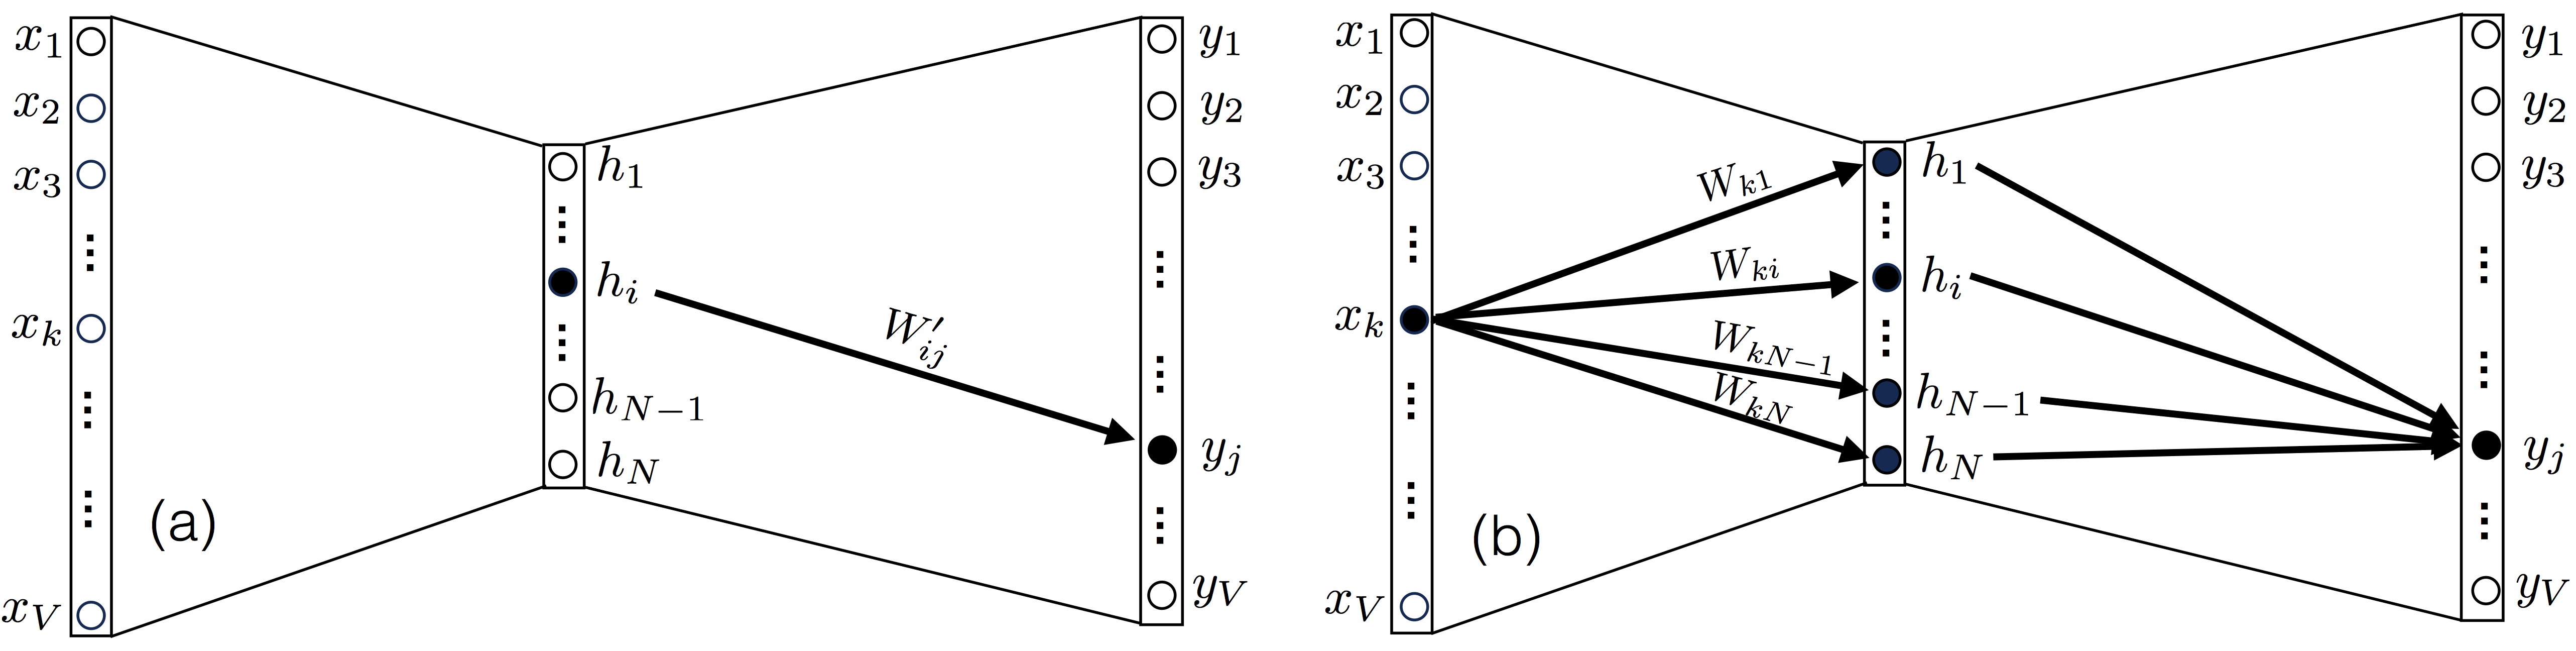
\includegraphics[width=\linewidth,keepaspectratio]{w2v13}
\end{center} 

\end{frame}

%%%%%%%%%%%%%%%%%%%%%%%%%%%%%%%%%%%%%%%%%%%%%%%%%%%%%%%%%%%%%%%%%%%%%%%%%%%%%%%%%%
\begin{frame}[fragile]\frametitle{The backpropagation algorithm for the CBOW model}
Hence, among all the derivatives $\partial u_k/\partial W'_{ij}$, only the one where $k=j$ will be different from zero. In other words,

\begin{equation}
\frac{\partial\mathcal{L}}{\partial W'_{ij}} = \frac{\partial\mathcal{L}}{\partial u_j}\frac{\partial u_j}
{\partial W'_{ij}}
\label{eq:derivative}
\end{equation}

For $\partial \mathcal{L}/\partial u_j$

\begin{equation}
\frac{\partial\mathcal{L}}{\partial u_j} = -\delta_{jj^*} + y_j := e_j
\label{eq:term}
\end{equation}

Where, $\delta_{jj^*}$ is a Kronecker delta: it is equal to 1 if $j=j^*$, otherwise 0.

$e$ is the difference between the target (label) and the predicted output, i.e., it is the prediction error vector


\end{frame}


%%%%%%%%%%%%%%%%%%%%%%%%%%%%%%%%%%%%%%%%%%%%%%%%%%%%%%%%%%%%%%%%%%%%%%%%%%%%%%%%%%
\begin{frame}[fragile]\frametitle{The backpropagation algorithm for the CBOW model}

For the second term on the right hand side of eq.\ref{eq:derivative}, we have

\begin{equation}
\frac{\partial u_j}{\partial W'_{ij}} = \sum_{k=1}^V W_{ik}x_k
\label{eq:term}
\end{equation}

After inserting eqs.\ref{eq:term} and \ref{eq:term} into eq. \ref{eq:derivative}, we obtain

\begin{equation}
% \bbox[white,5px,border:2px dotted red]{
\frac{\partial\mathcal{L}}{\partial W'_{ij}} = (-\delta_{jj^*} + y_j) \left(\sum_{k=1}^V W_{ki}x_k\right)
% }
\label{eq:backprop1}
\end{equation}


\end{frame}

%%%%%%%%%%%%%%%%%%%%%%%%%%%%%%%%%%%%%%%%%%%%%%%%%%%%%%%%%%%%%%%%%%%%%%%%%%%%%%%%%%
\begin{frame}[fragile]\frametitle{The backpropagation algorithm for the CBOW model}

  \begin{itemize}
    \item We can go through a similar exercise for the derivative $\partial\mathcal{L}/\partial W_{ij}$
	\item however this time we note that after fixing the input $x_k$ 
the output $y_i$ and node $j$ depends on all the elements of the matrix $W$ that are connected to the input
\item Therefore, this time we have to retain all the elements in the sum. 
\item Element $u_k$ of the vector $u$ as 
\end{itemize}

  \begin{equation*}
u_k = \sum_{m=1}^N\sum_{l=1}^VW'_{mk}W_{lm}x_l\ .
\end{equation*}

From this equation it is then easy to write down $\partial u_k/\partial W_{ij}$
since the only term that survives from the derivation will be the one in which $l=i$ and $m=j$ or 

\begin{equation}
\frac{\partial u_k}{\partial W_{ij}} = W'_{jk}x_i\  .
\label{eq:term}
\end{equation}

\end{frame}



%%%%%%%%%%%%%%%%%%%%%%%%%%%%%%%%%%%%%%%%%%%%%%%%%%%%%%%%%%%%%%%%%%%%%%%%%%%%%%%%%%
\begin{frame}[fragile]\frametitle{Vectorization}
We can simplify the notation of eqs. \ref{eq:backprop1} and \ref{eq:backprop2} by using a vector notation. Doing so, we obtain for eq. \ref{eq:backprop1}

\begin{equation}
% \bbox[white,5px,border:2px dotted red]{
\frac{\partial\mathcal{L}}{\partial W'} =  (W^T\textbf{x}) \otimes \textbf{e}
% }
\end{equation}

where the symbol $\otimes$ denotes the outer product, that in Python can be obtained using the numpy.outer method.

For eq. \ref{eq:backprop2} we obtain

\begin{equation}
% \bbox[white,5px,border:2px dotted red]{
\frac{\partial \mathcal{L}}{\partial W} = \textbf{x}\otimes(W'\textbf{e})
% }
\end{equation}

 
\end{frame}

%%%%%%%%%%%%%%%%%%%%%%%%%%%%%%%%%%%%%%%%%%%%%%%%%%%%%%%%%%%%%%%%%%%%%%%%%%%%%%%%%%
\begin{frame}[fragile]\frametitle{Applying these results to gradient descent}

 In order to apply gradient descent, after fixing a learning rate 
$\eta>0$
 we can update the values of the weight vectors by using the equations
 
 \begin{eqnarray}
W_{\textrm{new}} & = W_{\textrm{old}} - \eta \frac{\partial \mathcal{L}}{\partial W} \nonumber \\
W'_{\textrm{new}} & = W'_{\textrm{old}} - \eta \frac{\partial \mathcal{L}}{\partial W'} \nonumber \\
\end{eqnarray}

\end{frame}


%%%%%%%%%%%%%%%%%%%%%%%%%%%%%%%%%%%%%%%%%%%%%%%%%%%%%%%%%%%%%%%%%%%%%%%%%%%%%%%%%%
\begin{frame}[fragile]\frametitle{Iterating the algorithm}

  \begin{itemize}
    \item In order to conclude the first pass, we have to go through all our training examples. 
	\item Once we do this, we will have gone through a full epoch of optimization. 
	\item At that point, most likely we will need to start again iterating through all our training data, until we reach a point in which we don’t observe big changes in the loss function. 
	\item At that point, we can stop and declare that our neural network has been trained!
	  \end{itemize}

\end{frame}






%%%%%%%%%%%%%%%%%%%%%%%%%%%%%%%%%%%%%%%%%%%%%%%%%%%%%%%%%%%%%%%%%%%%%%%%%%%%%%%%%%
\begin{frame}[fragile]\frametitle{}

\begin{center}
{\Large Working with an Example}

{\tiny (Ref:The back-propagation algorithm for Word2Vec - Marginalia )}

\end{center}

\end{frame}

%%%%%%%%%%%%%%%%%%%%%%%%%%%%%%%%%%%%%%%%%%%%%%%%%%%%%%%%%%%%%%%%%%%%%%%%%%%%%%%%%%
\begin{frame}[fragile]\frametitle{Problem Info}
  \begin{itemize}
    \item Text corpus: ``I like playing football''
	\item 4 words, so vocabulary for this problem is of dimension 4 ($V=4$). Each of the word
	\item $\textrm{Vocabulary}=[\textrm{“I”},  \textrm{“like”}, \textrm{“playing”}, \textrm{“football”}]$
	\item We decide tho have $N=2$
	\item Our neural network will look like this:
  \end{itemize}
  
\begin{center}
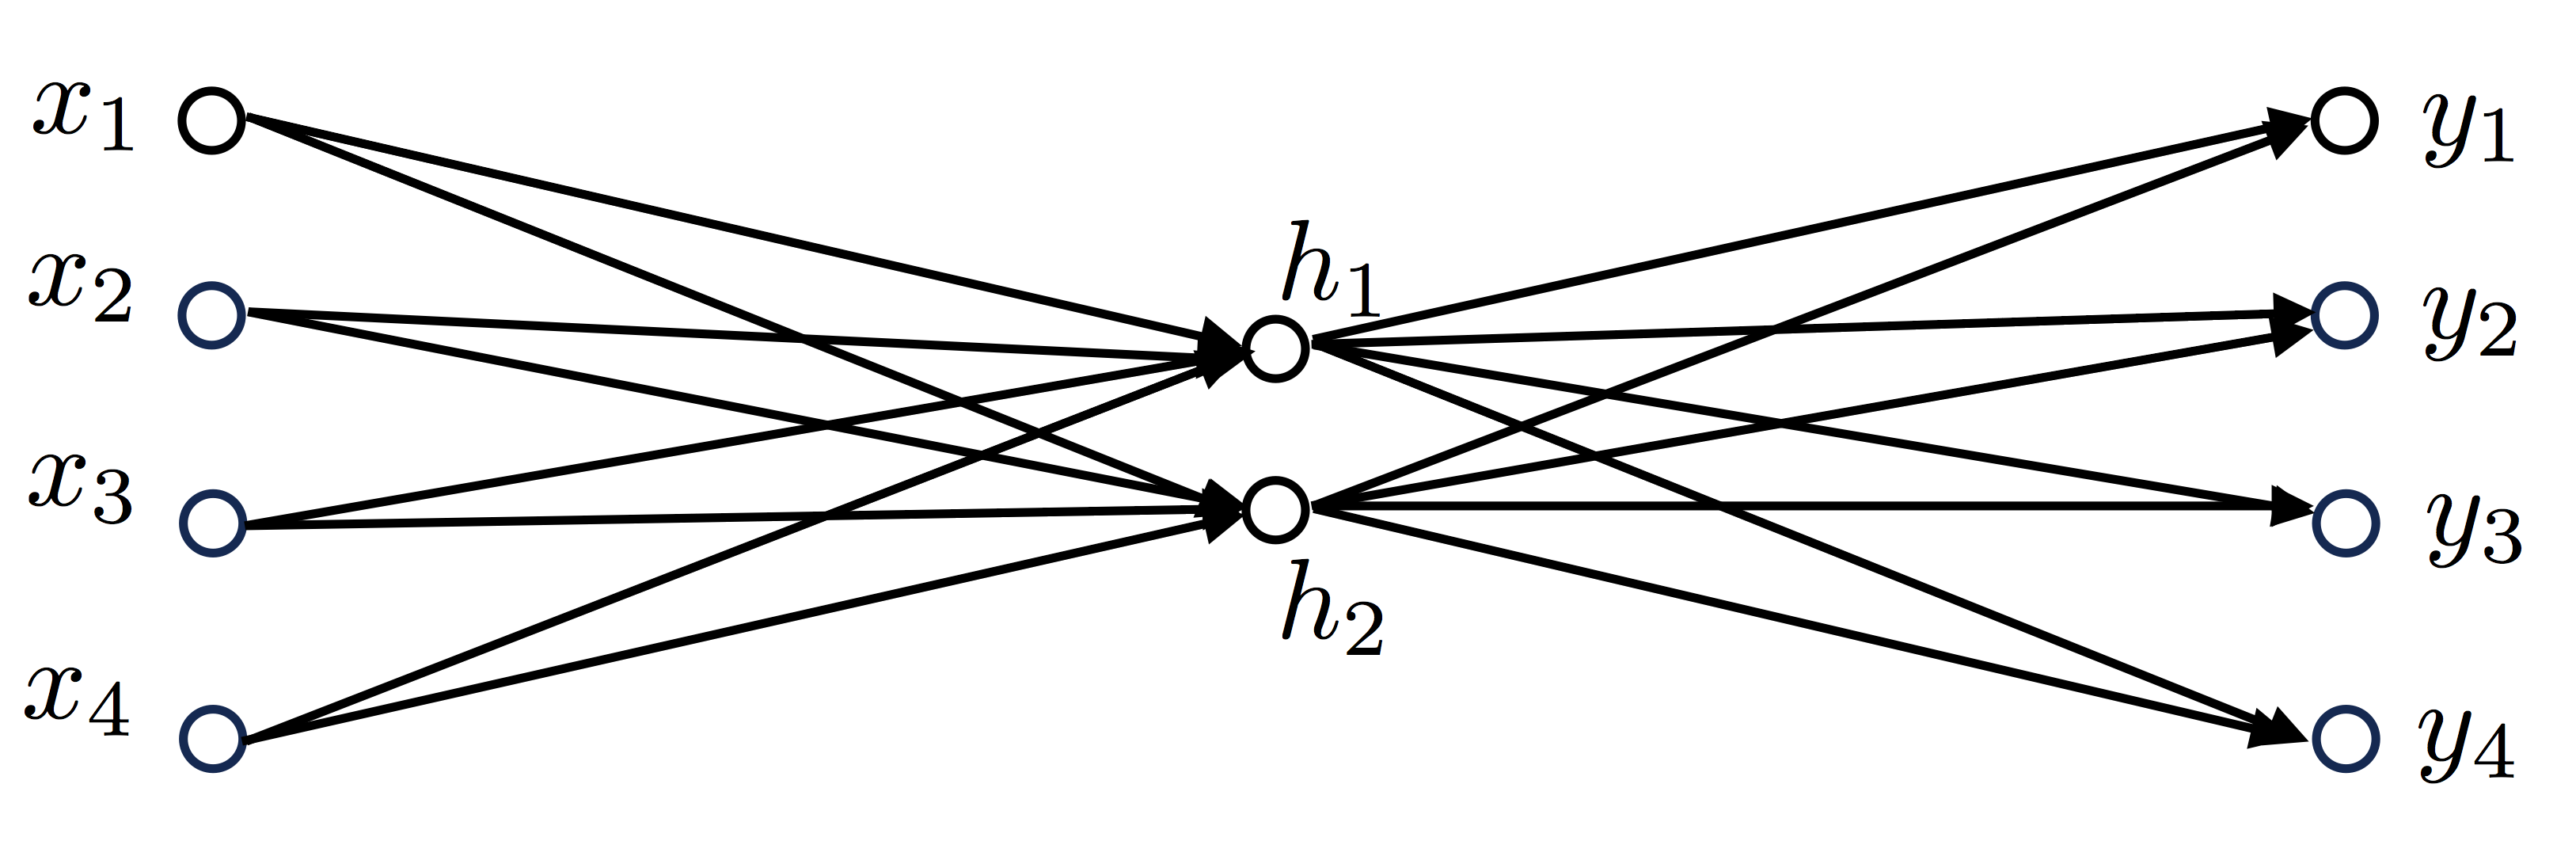
\includegraphics[width=0.6\linewidth,keepaspectratio]{w2v8}
\end{center}  
  
\end{frame}

%%%%%%%%%%%%%%%%%%%%%%%%%%%%%%%%%%%%%%%%%%%%%%%%%%%%%%%%%%%%%%%%%%%%%%%%%%%%%%%%%%
\begin{frame}[fragile]\frametitle{Input Output}
  \begin{itemize}
    \item  ``target word'' the word that follows a given word in the text (which becomes our ``context word'' or input word).
	\item For example, the target word for the context word “like” will be the word “playing”. 
  \end{itemize}
  
\begin{center}
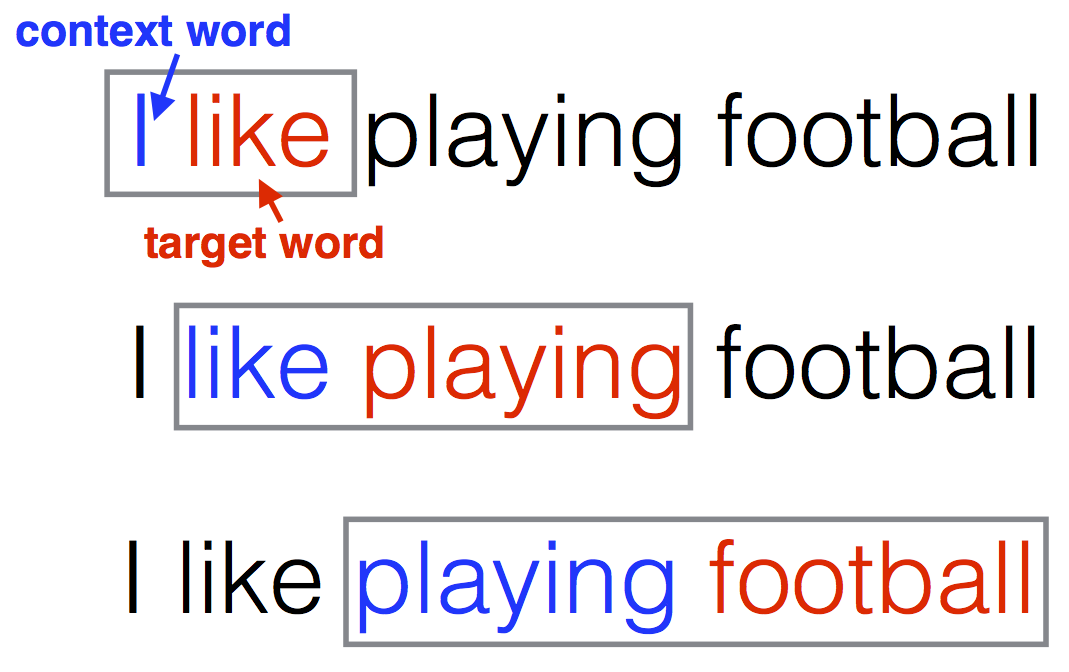
\includegraphics[width=0.45\linewidth,keepaspectratio]{w2v10}
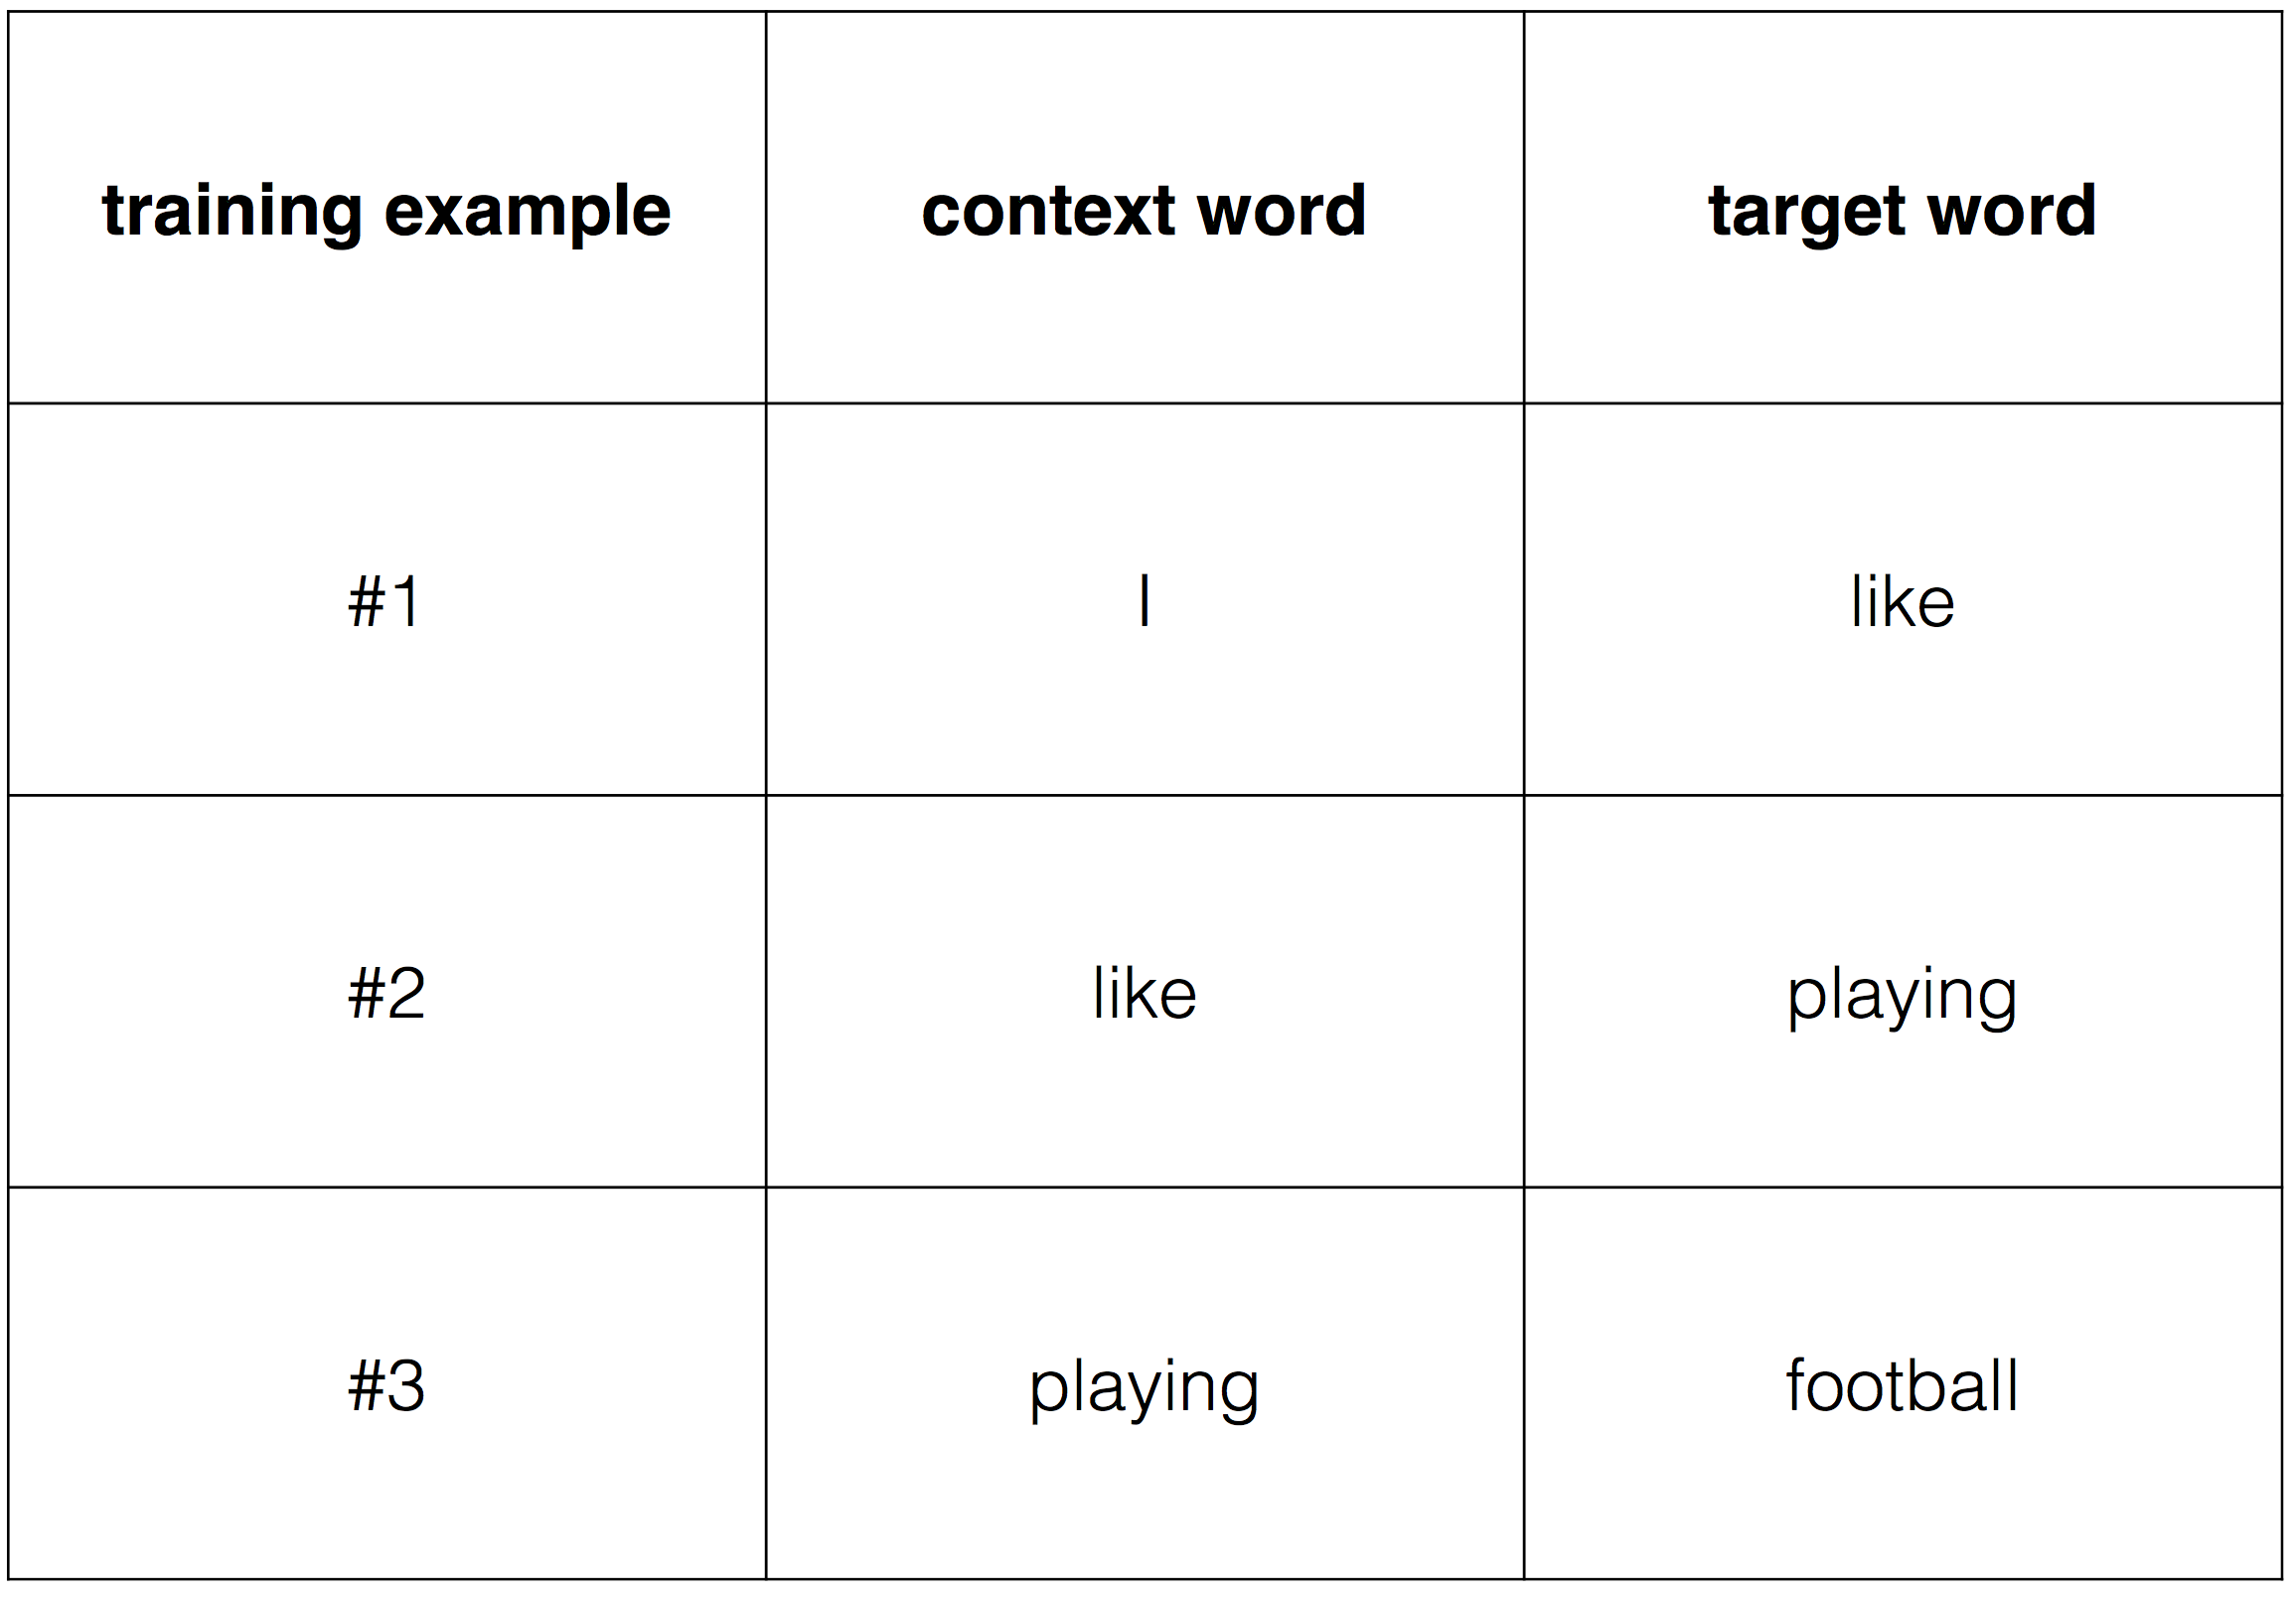
\includegraphics[width=0.45\linewidth,keepaspectratio]{w2v11}
\end{center}  
  
\end{frame}

%%%%%%%%%%%%%%%%%%%%%%%%%%%%%%%%%%%%%%%%%%%%%%%%%%%%%%%%%%%%%%%%%%%%%%%%%%%%%%%%%%
\begin{frame}[fragile]\frametitle{Input Output}
Each word gets one-hot vector.
  \begin{itemize}
    \item “I” : $[1, 0, 0, 0]$
	\item “like” : $[0, 1, 0, 0]$
	\item So on and also the same would be for the target words
  \end{itemize}
  
\begin{center}
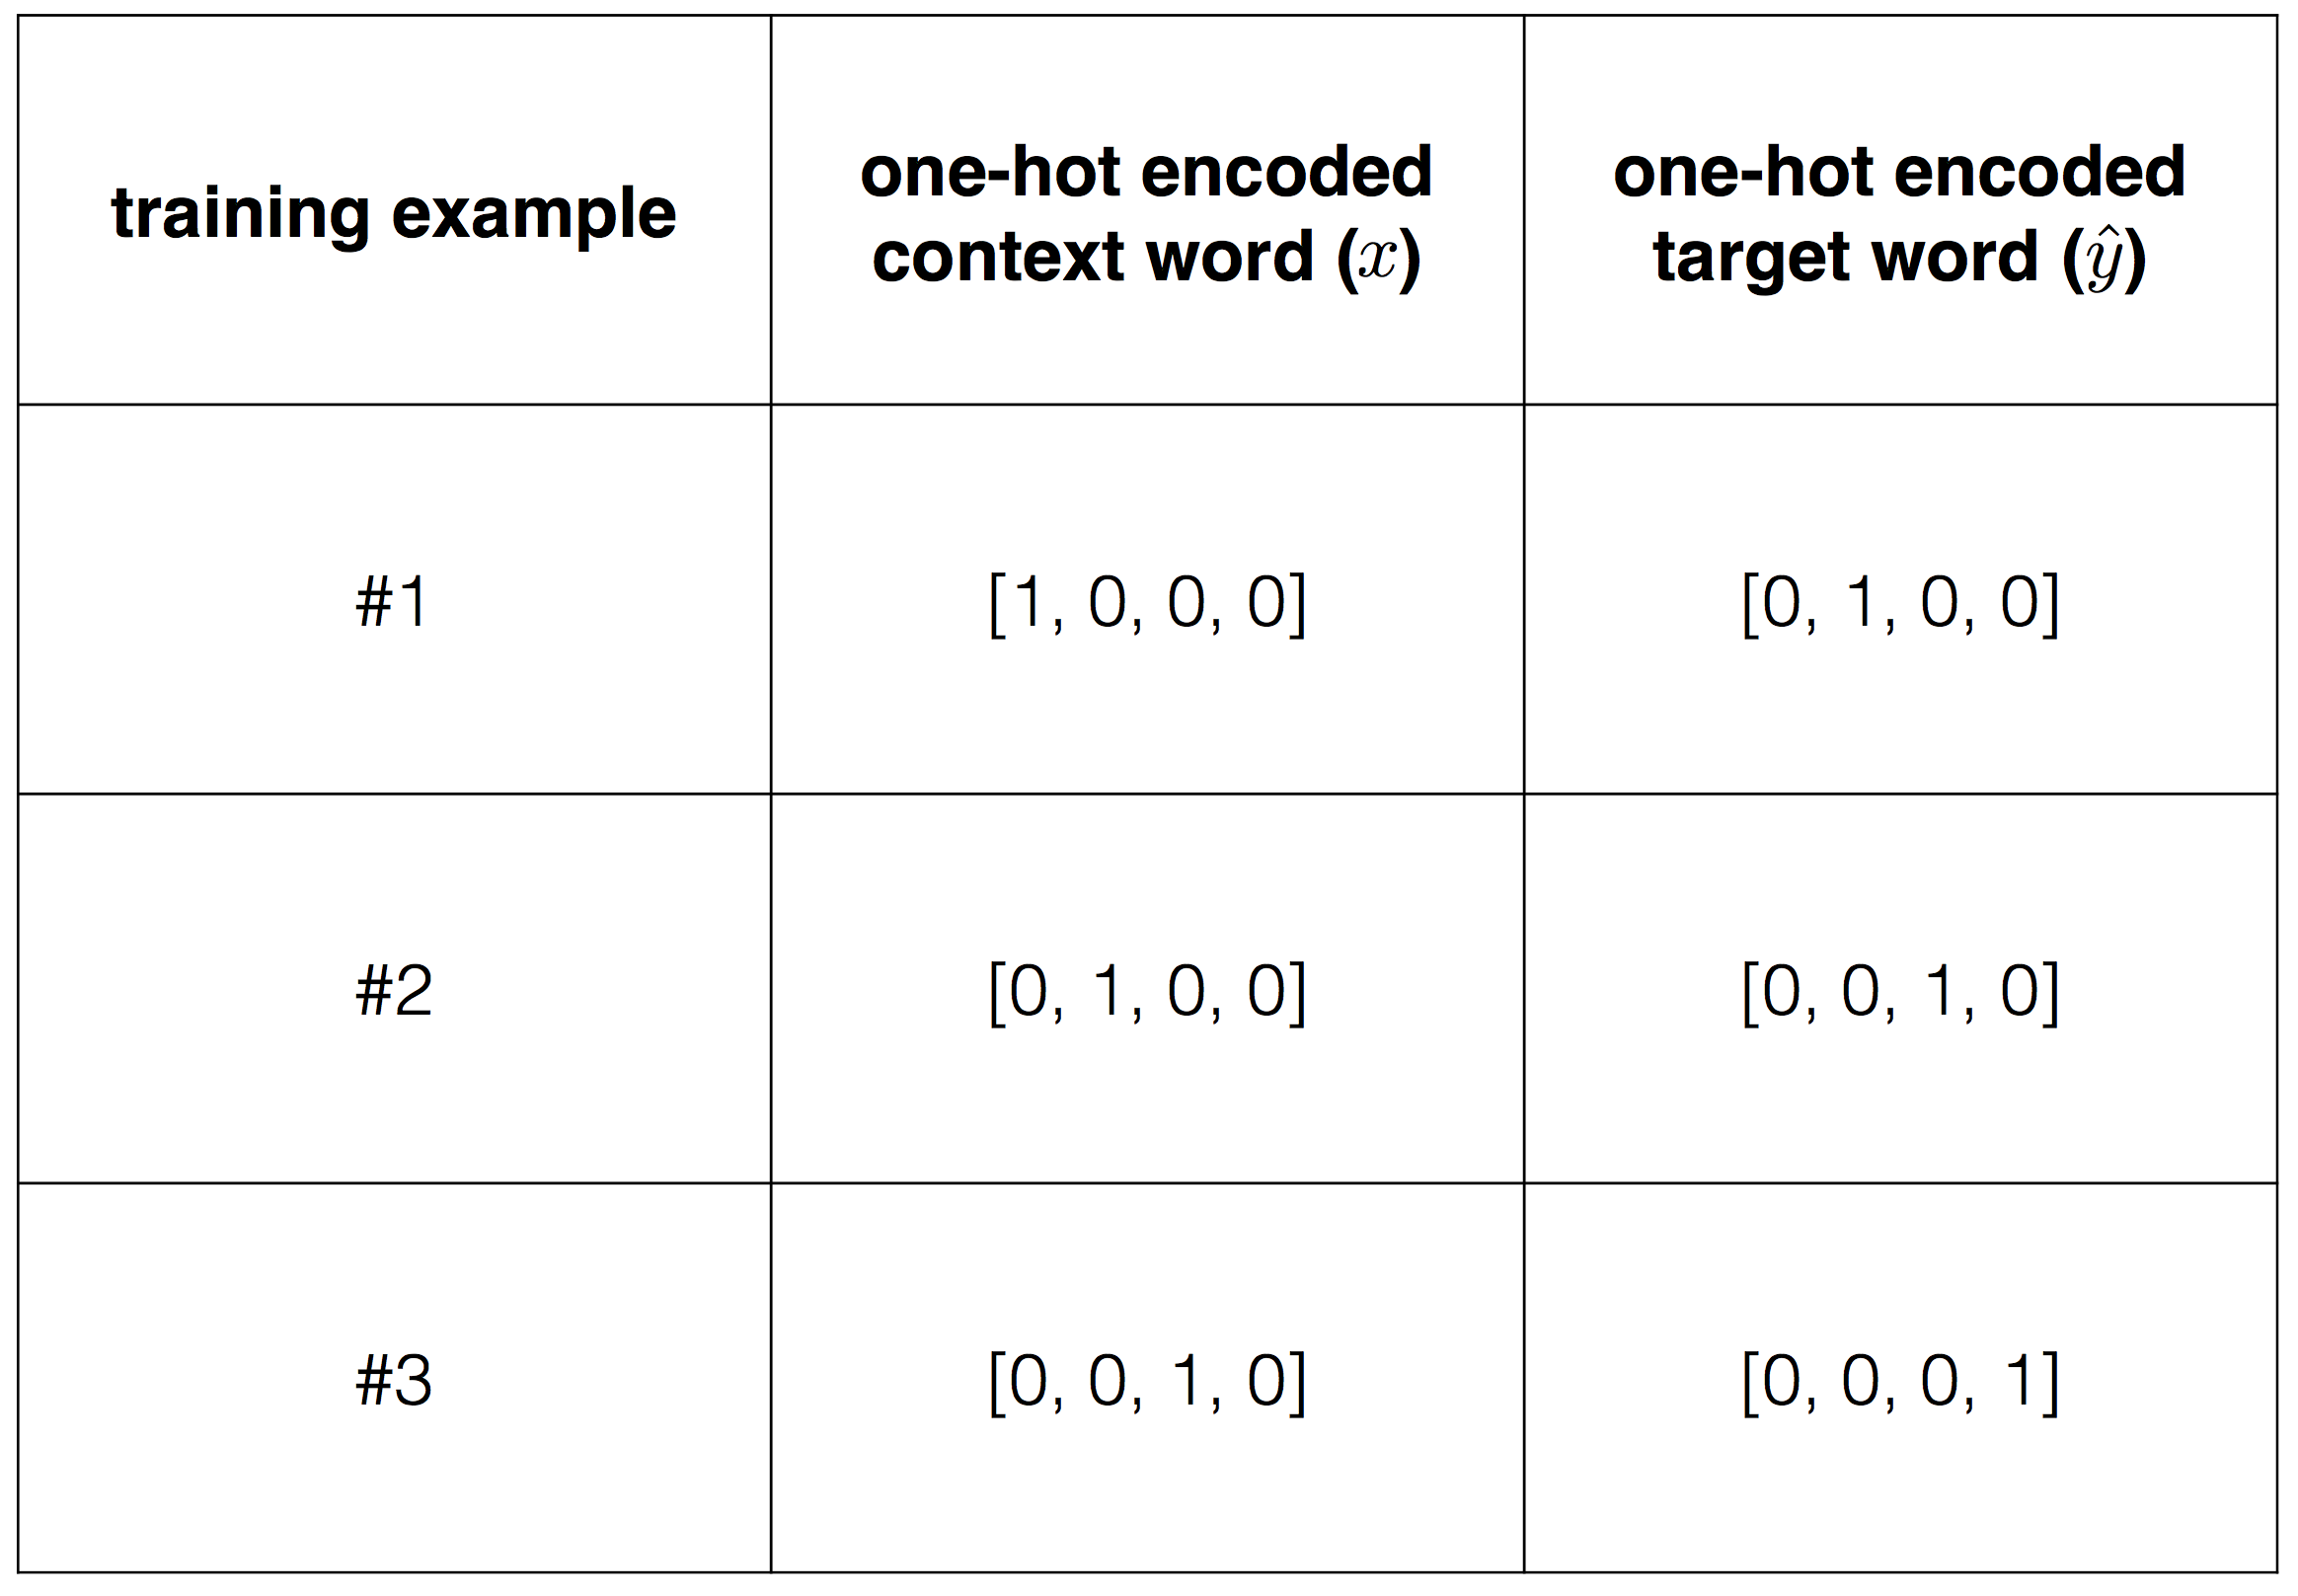
\includegraphics[width=0.6\linewidth,keepaspectratio]{w2v12}
\end{center}    

  
\end{frame}

%%%%%%%%%%%%%%%%%%%%%%%%%%%%%%%%%%%%%%%%%%%%%%%%%%%%%%%%%%%%%%%%%%%%%%%%%%%%%%%%%%
\begin{frame}[fragile]\frametitle{Training}
  \begin{itemize}
    \item At this point we want to train our model, finding the weights that minimize the loss function. 
	\item This corresponds to finding the weights that, given a context vector, can predict with the highest accuracy what is the corresponding target word $\hat{y}$
	\item Lets say we have first data point: the context word is “I” and the target word is “like”. 
	\item Ideally, the values of the weights should be such that 
	\item when the input $\textbf{x}=(1, 0, 0, 0)$  - which corresponds to the word “I” 
	\item then the output will be close to  $\hat{\textbf{y}}=(0, 1, 0, 0)$  - which corresponds to the word “like”.
  \end{itemize}
 
\end{frame}

%%%%%%%%%%%%%%%%%%%%%%%%%%%%%%%%%%%%%%%%%%%%%%%%%%%%%%%%%%%%%%%%%%%%%%%%%%%%%%%%%%
\begin{frame}[fragile]\frametitle{Weight Matrices}
  \begin{itemize}
    \item We either initialize weight matrices with random numbers or  standard normal distribution.

\item Say, the initial state of $W$, which is a $4 \times 2$ matrix, is
\item $W =
\begin{pmatrix}
	-1.38118728 &  0.54849373 \\
	0.39389902  &  -1.1501331	\\
	-1.16967628 &  0.36078022 \\
	0.06676289  &  -0.14292845
\end{pmatrix}
$

\item and the initial state of $W$, which is a $2 \times 4$ matrix, is

\item $
W' =
\begin{pmatrix}
	1.39420129	& -0.89441757 &  0.99869667 &  0.44447037 \\
	0.69671796 & -0.23364341 & 0.21975196 & -0.0022673
\end{pmatrix}
$

\end{itemize}

\end{frame}

%%%%%%%%%%%%%%%%%%%%%%%%%%%%%%%%%%%%%%%%%%%%%%%%%%%%%%%%%%%%%%%%%%%%%%%%%%%%%%%%%%
\begin{frame}[fragile]\frametitle{First Training Data}
  \begin{itemize}
    \item For the first training data “I like”, with context word $\textbf{x}=(1,0,0,0)^T$ nd target word $\hat{\textbf{y}}=(0,0,1,0)^T$  , we have
	
$\textbf{h} = W^T\textbf{x}=
\begin{pmatrix}
	-1.38118728	\\
	0.54849373
\end{pmatrix}
$
\item Then we have

$
\textbf{u} = W'^T\textbf{h}=
\begin{pmatrix}
	-1.54350765  \\
	1.10720623 \\
	-1.25885456 \\
	-0.61514042
\end{pmatrix}
$
\item and finally
$
\textbf{y} = \mathbb{S}\textrm{oftmax}(\textbf{u})=
\begin{pmatrix}
	0.05256567 \\
	 0.7445479  \\
	 0.06987559 \\
	 0.13301083
\end{pmatrix}
$
\end{itemize}

\end{frame}

%%%%%%%%%%%%%%%%%%%%%%%%%%%%%%%%%%%%%%%%%%%%%%%%%%%%%%%%%%%%%%%%%%%%%%%%%%%%%%%%%%
\begin{frame}[fragile]\frametitle{Loss Function}
  \begin{itemize}
    \item At this first iteration, the loss function will be the negative logarithm of the second element of $y$ (becuase thats the target ``1''):
	
	$\mathcal{L}=-\log\mathbb{P}(\textrm{“like”}|\textrm{“I”})=-\log y_3 = -\log(0.7445479)= 0.2949781.$ 
	\item We could also calculate it using eq. \ref{eq:loss} , like so:
	
\begin{eqnarray*}
\mathcal{L}=-u_2+\log\sum_{i=1}^4 u_i=-1.10720623 + \\
\log[\exp(-1.54350765)+\exp(1.10720623) \\ 
+\exp(-1.25885456)+ \\
\exp(-0.61514042)]=0.2949781.
\end{eqnarray*}
\item At this point, before going into the next training example (“like”, “playing”), we have to change the weights of the network using gradient descent. 
\item How to do this? 
\item The backpropagation algorithm is the answer!
\end{itemize}

\end{frame}

% %%%%%%%%%%%%%%%%%%%%%%%%%%%%%%%%%%%%%%%%%%%%%%%%%%%
% \begin{frame}[fragile] \frametitle{Skip Gram}

% \begin{center}
% 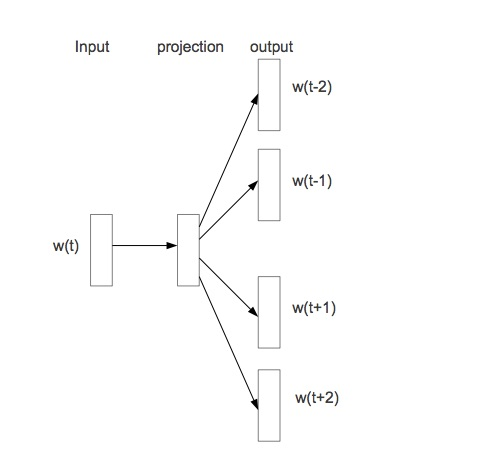
\includegraphics[width=0.6\linewidth,keepaspectratio]{skipGram.jpg}
% \end{center}

% \end{frame}

% %%%%%%%%%%%%%%%%%%%%%%%%%%%%%%%%%%%%%%%%%%%%%%%%%%%
% \begin{frame}[fragile] \frametitle{Skip Gram Weights}

% \begin{center}
% 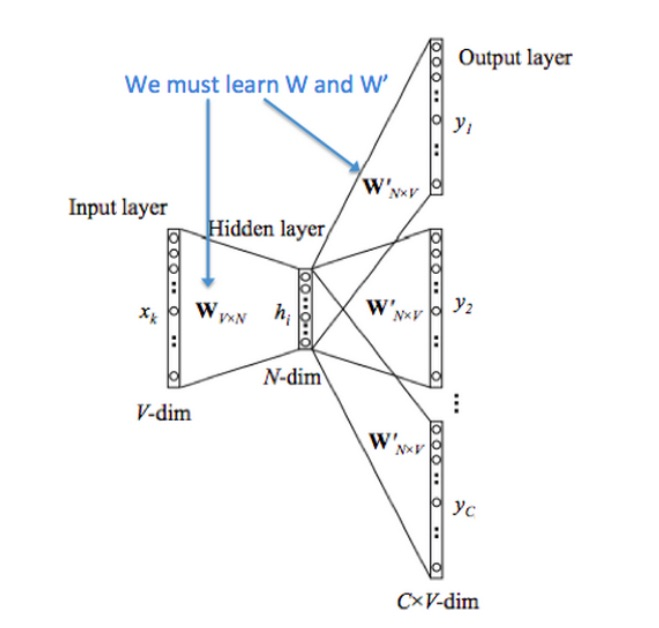
\includegraphics[width=0.6\linewidth,keepaspectratio]{skipGram2.jpg}
% \end{center}

% \end{frame}


% %%%%%%%%%%%%%%%%%%%%%%%%%%%%%%%%%%%%%%%%%%%%%%%%%%%
% \begin{frame}[fragile] \frametitle{Continuous Bag Of Words}

% \begin{center}
% 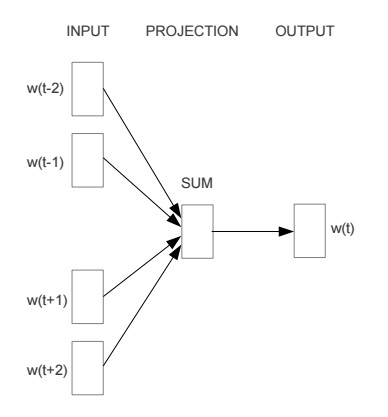
\includegraphics[width=0.6\linewidth,keepaspectratio]{continuousBagOfWords.jpg}
% \end{center}

% \end{frame}

% %%%%%%%%%%%%%%%%%%%%%%%%%%%%%%%%%%%%%%%%%%%%%%%%%%%
% \begin{frame}[fragile] \frametitle{Continuous Bag Of Words Weights}

% \begin{center}
% 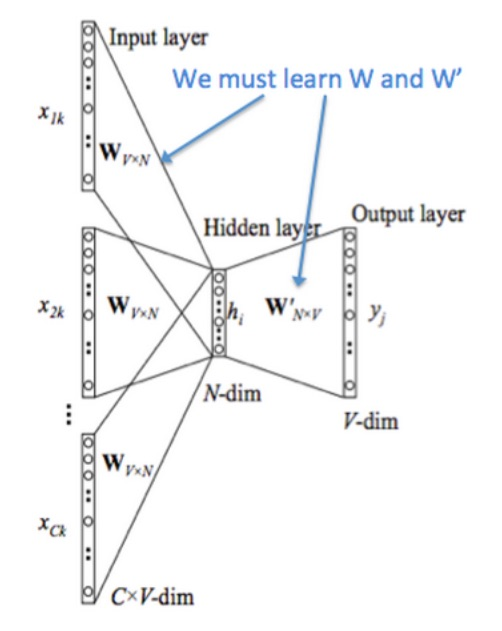
\includegraphics[width=0.4\linewidth,keepaspectratio]{continuousBagOfWords2.jpg}
% \end{center}

% \end{frame}


% %%%%%%%%%%%%%%%%%%%%%%%%%%%%%%%%%%%%%%%%%%%%%%%%%%%%%%%%%%%%%%%%%%%%%%%%%%%%%%%%%%
% \begin{frame}[fragile]\frametitle{BoW}
  % \begin{itemize}
  % \item  Text as a sequence of: Characters, \textbf{words}, Phrases and named entities, Sentences, Paragraphs, \ldots
    % \item Each unique word has BOW one hot encoded vector representation
  % \end{itemize}
  % \begin{center}
% 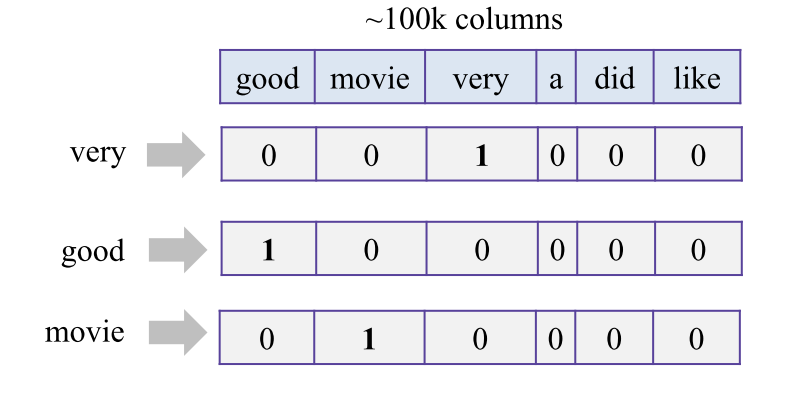
\includegraphics[width=0.6\linewidth,keepaspectratio]{classdl1}
% \end{center}

% (Ref: https://www.coursera.org/learn/language-processing/lecture/UqVpR/neural-networks-for-words)
% \end{frame}


% %%%%%%%%%%%%%%%%%%%%%%%%%%%%%%%%%%%%%%%%%%%%%%%%%%%%%%%%%%%%%%%%%%%%%%%%%%%%%%%%%%
% \begin{frame}[fragile]\frametitle{BoW}
  % \begin{itemize}
    % \item How to get aggregate for the whole sentence?
    % \item Sum all up.
  % \end{itemize}
  % \begin{center}
% 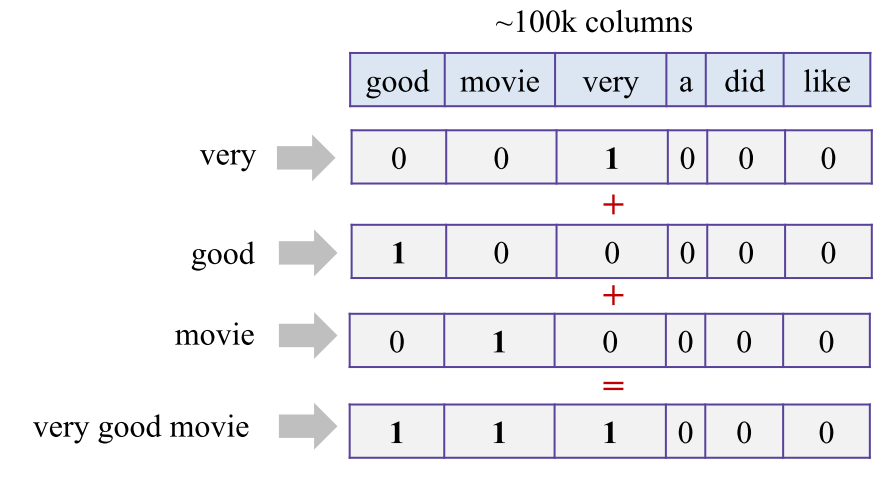
\includegraphics[width=0.6\linewidth,keepaspectratio]{classdl2}
% \end{center}
% Very sparse. But in Deep Learning we like Dense reprentation.

% (Ref: https://www.coursera.org/learn/language-processing/lecture/UqVpR/neural-networks-for-words)
% \end{frame}



% %%%%%%%%%%%%%%%%%%%%%%%%%%%%%%%%%%%%%%%%%%%%%%%%%%%%%%%%%%%%%%%%%%%%%%%%%%%%%%%%%%
% \begin{frame}[fragile]\frametitle{BoW}
  % \begin{itemize}

    % \item Dense with around 300 real values.
    % \item Pre-trained embeddings in unsupervised manner.
    % \item Words with similar (+/-ve) context are near in n-dimensional space.    
  % \end{itemize}
  % \begin{center}
% 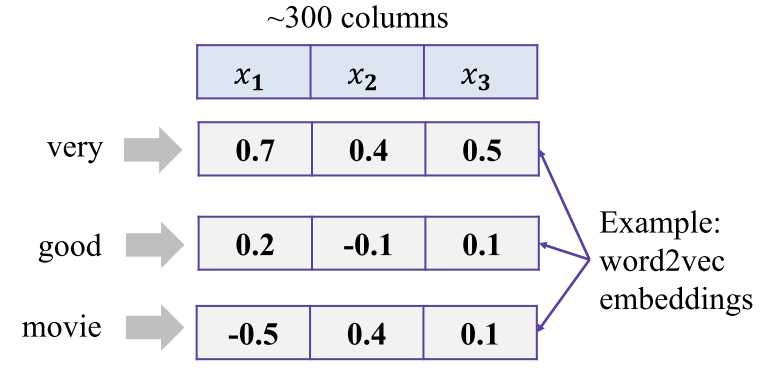
\includegraphics[width=0.6\linewidth,keepaspectratio]{classdl3}
% \end{center}

% (Ref: https://www.coursera.org/learn/language-processing/lecture/UqVpR/neural-networks-for-words)
% \end{frame}

% %%%%%%%%%%%%%%%%%%%%%%%%%%%%%%%%%%%%%%%%%%%%%%%%%%%%%%%%%%%%%%%%%%%%%%%%%%%%%%%%%%
% \begin{frame}[fragile]\frametitle{BoW}
  % \begin{itemize}
    % \item How to get aggregate for the whole sentence?
    % \item Sum all up.
  % \end{itemize}
  % \begin{center}
% 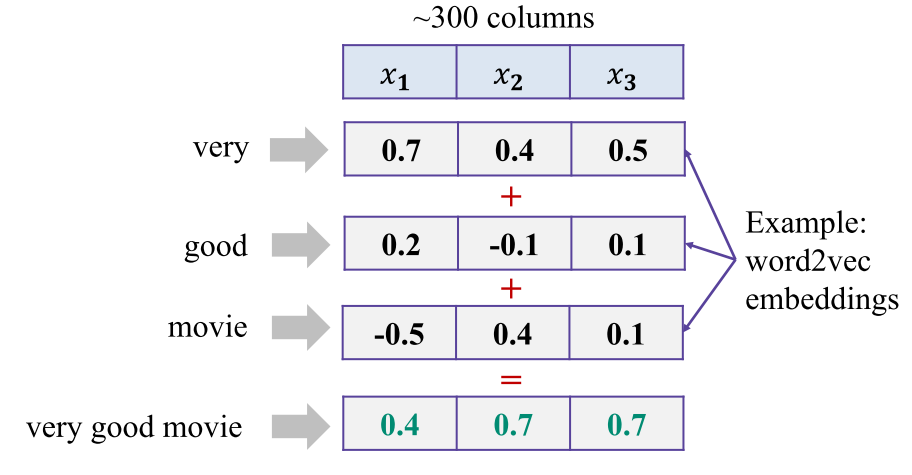
\includegraphics[width=0.6\linewidth,keepaspectratio]{classdl4}
% \end{center}

% (Ref: https://www.coursera.org/learn/language-processing/lecture/UqVpR/neural-networks-for-words)
% \end{frame}


% %%%%%%%%%%%%%%%%%%%%%%%%%%%%%%%%%%%%%%%%%%%%%%%%%%%%%%%%%%%%%%%%%%%%%%%%%%%%%%%%%%
% \begin{frame}[fragile]\frametitle{BoW}
% One word (unigram) examples:
  % \begin{center}
% 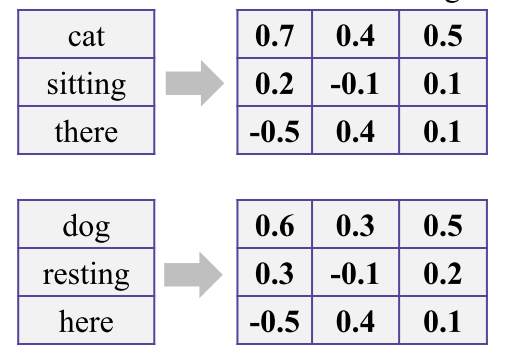
\includegraphics[width=0.6\linewidth,keepaspectratio]{classdl5}
% \end{center}

% (Ref: https://www.coursera.org/learn/language-processing/lecture/UqVpR/neural-networks-for-words)
% \end{frame}

% %%%%%%%%%%%%%%%%%%%%%%%%%%%%%%%%%%%%%%%%%%%%%%%%%%%%%%%%%%%%%%%%%%%%%%%%%%%%%%%%%%
% \begin{frame}[fragile]\frametitle{BoW}
  % \begin{itemize}
    % \item How to get word2vecs for Two words (bigrams), gen that word2vec is only for unigrams?
    % \item We can take pair of those two words and their vecs.
    % \item We can take convolution filter of same size (full match on top of each other)
    % \item Then compute dot product giving out single scalar number
  % \end{itemize}


% (Ref: https://www.coursera.org/learn/language-processing/lecture/UqVpR/neural-networks-for-words)
% \end{frame}

% %%%%%%%%%%%%%%%%%%%%%%%%%%%%%%%%%%%%%%%%%%%%%%%%%%%%%%%%%%%%%%%%%%%%%%%%%%%%%%%%%%
% \begin{frame}[fragile]\frametitle{BoW}
  % \begin{center}
% 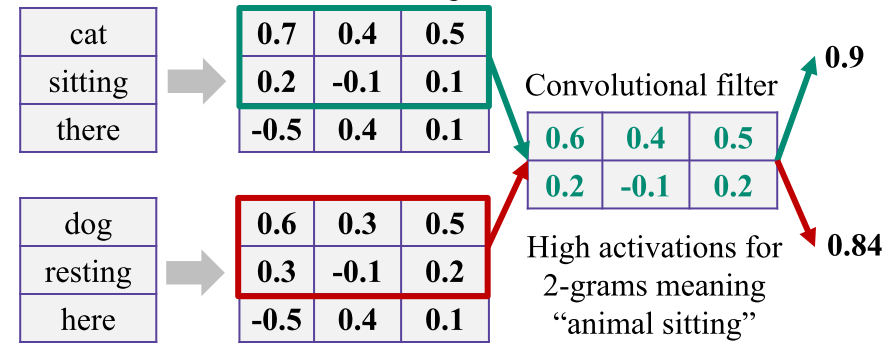
\includegraphics[width=0.8\linewidth,keepaspectratio]{classdl6}
% \end{center}

% Similar bigrams result in similar output of bigrams, a new feature. High level meaning ``animal sitting''.

% (Ref: https://www.coursera.org/learn/language-processing/lecture/UqVpR/neural-networks-for-words)
% \end{frame}

% %%%%%%%%%%%%%%%%%%%%%%%%%%%%%%%%%%%%%%%%%%%%%%%%%%%%%%%%%%%%%%%%%%%%%%%%%%%%%%%%%%
% \begin{frame}[fragile]\frametitle{BoW}
  % \begin{itemize}
    % \item Can be extended to 3-grams, 4-grams, etc.
    % \item One filter is not enough, need to track many n-grams
    % \item Convolution window goes from top, and starts filling output column.
  % \end{itemize}
  % \begin{center}
% 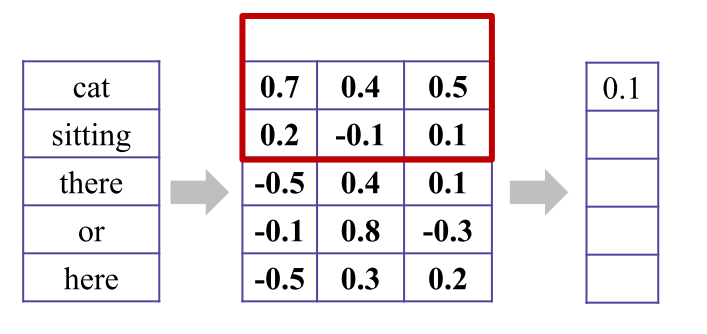
\includegraphics[width=0.6\linewidth,keepaspectratio]{classdl7}
% \end{center}

% (Ref: https://www.coursera.org/learn/language-processing/lecture/UqVpR/neural-networks-for-words)
% \end{frame}

% %%%%%%%%%%%%%%%%%%%%%%%%%%%%%%%%%%%%%%%%%%%%%%%%%%%%%%%%%%%%%%%%%%%%%%%%%%%%%%%%%%
% \begin{frame}[fragile]\frametitle{BoW}
  % \begin{itemize}
    % \item Problem: as input sentences are of variable lengths, the output will of same, ie variable length.

    % \item We CANNOT have any feature vector (row) of variable length
        % \item Relax the rule, nstead of all the valies, pick the max value, called max pooling
  % \end{itemize}
  % \begin{center}
% 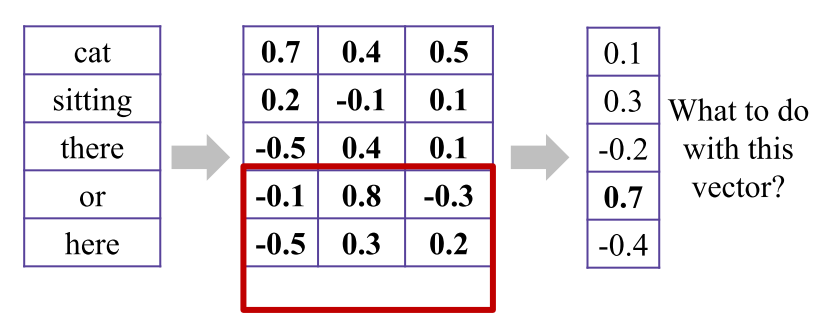
\includegraphics[width=0.6\linewidth,keepaspectratio]{classdl8}
% \end{center}

% (Ref: https://www.coursera.org/learn/language-processing/lecture/UqVpR/neural-networks-for-words)
% \end{frame}

% %%%%%%%%%%%%%%%%%%%%%%%%%%%%%%%%%%%%%%%%%%%%%%%%%%%%%%%%%%%%%%%%%%%%%%%%%%%%%%%%%%
% \begin{frame}[fragile]\frametitle{Let’s train many filters}
  % \begin{itemize}
    % \item 3,4,5-gram windows (total 3) with 100 filters each
    % \item Neural network using these features, total 300
    % \item Accuracy 89.6\% compared to 86.3\% in Naive Bayes on some cutomer dataset (ref:https://arxiv.org/pdf/1408.5882.pdf)
  % \end{itemize}
  % \begin{center}
% 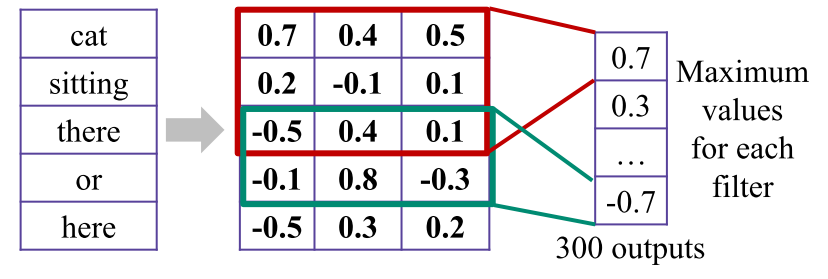
\includegraphics[width=0.9\linewidth,keepaspectratio]{classdl9}
% \end{center}

% (Ref: https://www.coursera.org/learn/language-processing/lecture/UqVpR/neural-networks-for-words)
% \end{frame}

% %%%%%%%%%%%%%%%%%%%%%%%%%%%%%%%%%%%%%%%%%%%%%%%%%%%%%%%%%%%%%%%%%%%%%%%%%%%%%%%%%%
% \begin{frame}[fragile]\frametitle{Summary}
  % \begin{itemize}
    % \item You can just average pre-trained word2vec vectors for your 
% text
    % \item You can do better with 1D convolutions that learn more 
% complex features
  % \end{itemize}


% (Ref: https://www.coursera.org/learn/language-processing/lecture/UqVpR/neural-networks-for-words)
% \end{frame}



% %%%%%%%%%%%%%%%%%%%%%%%%%%%%%%%%%%%%%%%%%%%%%%%%%%%
% \begin{frame}[fragile] \frametitle{}

% The specific implementation of these ideas by the Mikolov-headed
% group is known as word2vec. Gensim has pre-coded version of this.
% One can also build word vectors using own corpus.

% \end{frame}


% %%%%%%%%%%%%%%%%%%%%%%%%%%%%%%%%%%%%%%%%%%%%%%%%%%%
% \begin{frame}[fragile] \frametitle{}

% \begin{center}
% 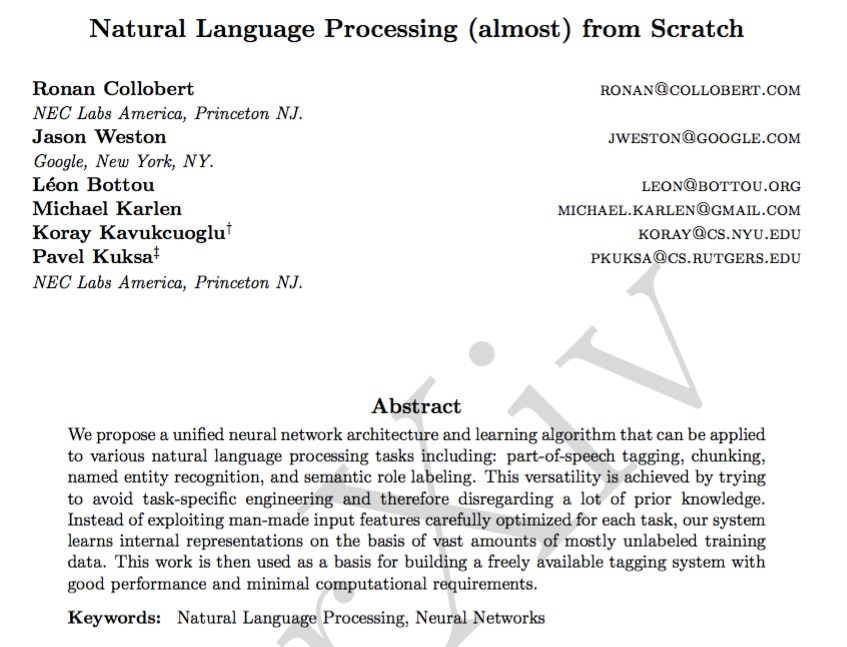
\includegraphics[height=8cm]{nlpScratch.jpg}
% \end{center}

% \end{frame}

% %%%%%%%%%%%%%%%%%%%%%%%%%%%%%%%%%%%%%%%%%%%%%%%%%%%%%%%%%%%%%%%%%%%%%%%%%%%%%%%%%%
% \begin{frame}[fragile]\frametitle{Characters}
  % \begin{itemize}
    % \item Text as a sequence of: \textbf{Characters}, words, Phrases and named entities, Sentences, Paragraphs, \ldots
% \item One hot encoding is managable here as number of characters + special symbols can be upto 70 say.
% \item Each character can be represneted by 70 ling one hot vector.

  % \end{itemize}
  % \begin{center}
% 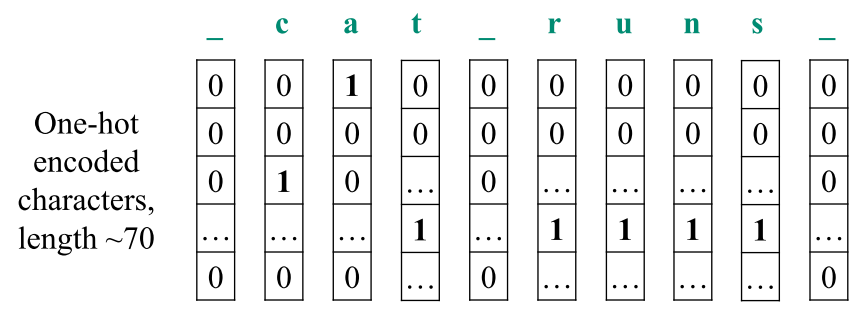
\includegraphics[width=0.6\linewidth,keepaspectratio]{classdl10}
% \end{center}

% (Ref: https://www.coursera.org/learn/language-processing/lecture/md0NM/neural-networks-for-characters)
% \end{frame}


% %%%%%%%%%%%%%%%%%%%%%%%%%%%%%%%%%%%%%%%%%%%%%%%%%%%%%%%%%%%%%%%%%%%%%%%%%%%%%%%%%%
% \begin{frame}[fragile]\frametitle{Characters}
  % \begin{itemize}
    % \item Convoltuion on it will result in a new vector.
    % \item We can employ different kernels and different vector can be generated.

  % \end{itemize}
  % \begin{center}
% 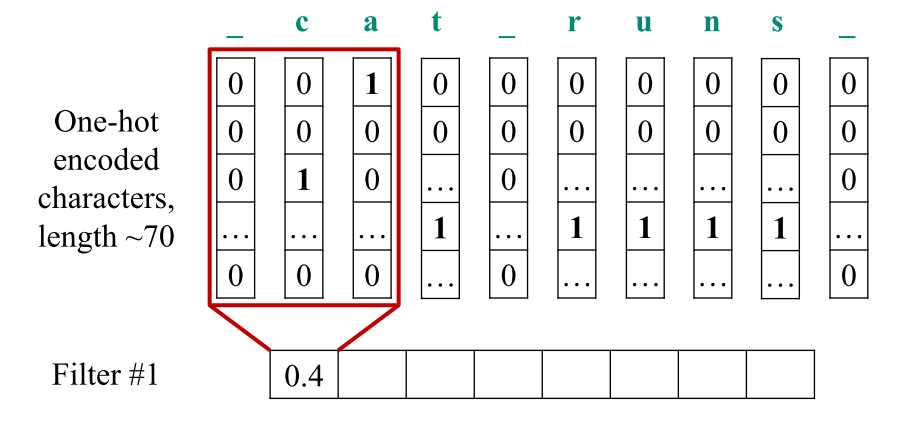
\includegraphics[width=0.6\linewidth,keepaspectratio]{classdl11}
% \end{center}

% (Ref: https://www.coursera.org/learn/language-processing/lecture/md0NM/neural-networks-for-characters)
% \end{frame}

% %%%%%%%%%%%%%%%%%%%%%%%%%%%%%%%%%%%%%%%%%%%%%%%%%%%%%%%%%%%%%%%%%%%%%%%%%%%%%%%%%%
% \begin{frame}[fragile]\frametitle{Characters}
  % \begin{itemize}
    % \item If we use 1024 kernels we will get 1024 filter vectors.
    % \item Need to apply pooling.
    % \item Pooling makes it position invariance.

  % \end{itemize}
  % \begin{center}
% 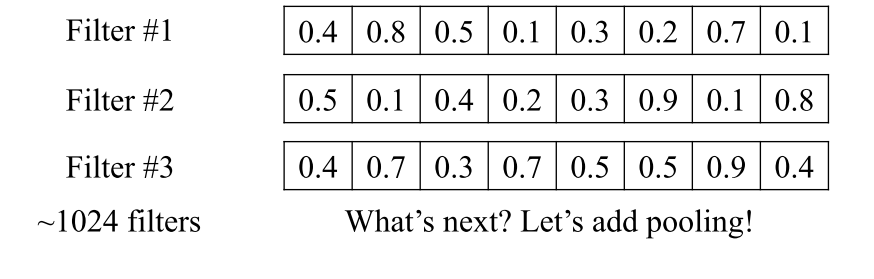
\includegraphics[width=0.6\linewidth,keepaspectratio]{classdl12}
% \end{center}

% (Ref: https://www.coursera.org/learn/language-processing/lecture/md0NM/neural-networks-for-characters)
% \end{frame}

% %%%%%%%%%%%%%%%%%%%%%%%%%%%%%%%%%%%%%%%%%%%%%%%%%%%%%%%%%%%%%%%%%%%%%%%%%%%%%%%%%%
% \begin{frame}[fragile]\frametitle{Characters}
  % \begin{itemize}
    % \item Get max of two (neighbours)

    % \item Move ahead with stride of 2, max again, and so on.

  % \end{itemize}
  % \begin{center}
% 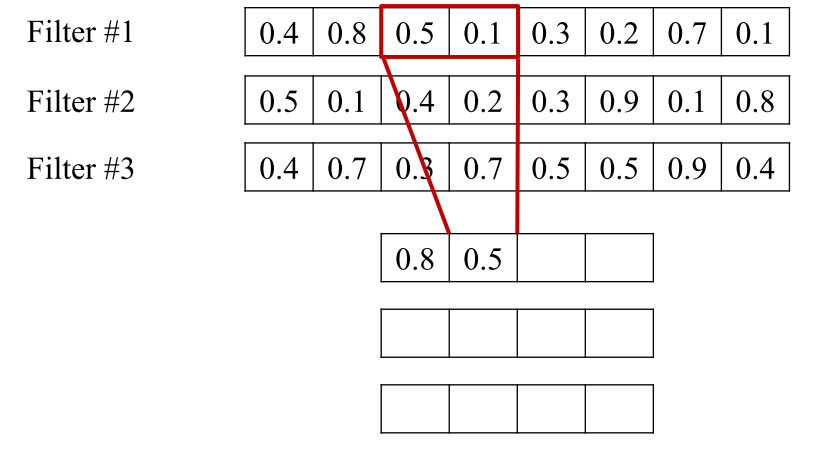
\includegraphics[width=0.6\linewidth,keepaspectratio]{classdl13}
% \end{center}

% (Ref: https://www.coursera.org/learn/language-processing/lecture/md0NM/neural-networks-for-characters)
% \end{frame}

% %%%%%%%%%%%%%%%%%%%%%%%%%%%%%%%%%%%%%%%%%%%%%%%%%%%%%%%%%%%%%%%%%%%%%%%%%%%%%%%%%%
% \begin{frame}[fragile]\frametitle{Characters}
  % \begin{itemize}
    % \item Repeat 1D convolution + pooling
  % \end{itemize}
  % \begin{center}
% 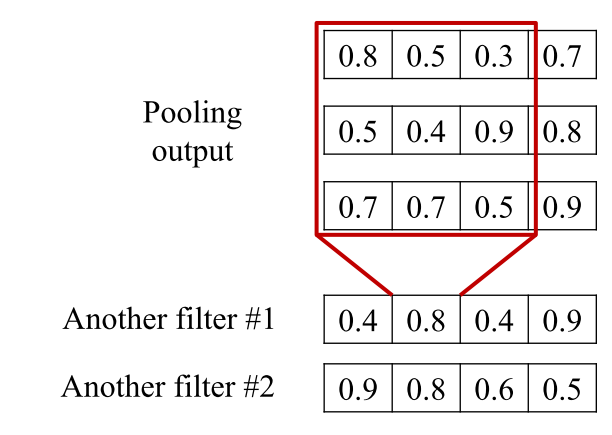
\includegraphics[width=0.6\linewidth,keepaspectratio]{classdl14}
% \end{center}

% (Ref: https://www.coursera.org/learn/language-processing/lecture/md0NM/neural-networks-for-characters)
% \end{frame}

% %%%%%%%%%%%%%%%%%%%%%%%%%%%%%%%%%%%%%%%%%%%%%%%%%%%%%%%%%%%%%%%%%%%%%%%%%%%%%%%%%%
% \begin{frame}[fragile]\frametitle{Characters}
  % \begin{itemize}
    	% \item Can repeat many times

  % \end{itemize}
  % \begin{center}
% 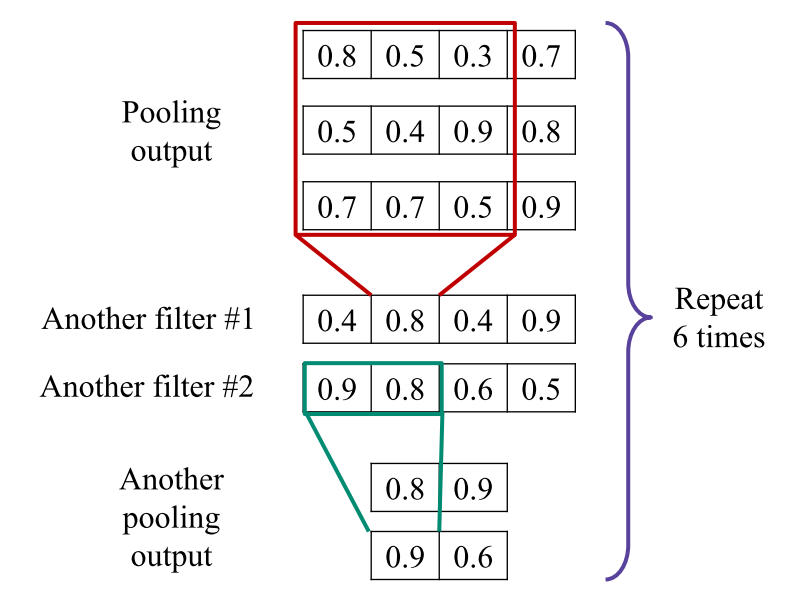
\includegraphics[width=0.6\linewidth,keepaspectratio]{classdl15}
% \end{center}

% (Ref: https://www.coursera.org/learn/language-processing/lecture/md0NM/neural-networks-for-characters)
% \end{frame}

% %%%%%%%%%%%%%%%%%%%%%%%%%%%%%%%%%%%%%%%%%%%%%%%%%%%%%%%%%%%%%%%%%%%%%%%%%%%%%%%%%%
% \begin{frame}[fragile]\frametitle{Model}
  % \begin{itemize}
   % \item  Let’s take only first 1014 characters of text
    % \item Apply 1D convolution + max pooling 6 times
    % \item  Kernels widths: 7, 7, 3, 3, 3, 3
    % \item Filters at each step: 1024
        % \item After that we have a 1024x34matrix of features
            % \item Apply MLP for your task

  % \end{itemize}


% (Ref: https://www.coursera.org/learn/language-processing/lecture/md0NM/neural-networks-for-characters)
% \end{frame}

% %%%%%%%%%%%%%%%%%%%%%%%%%%%%%%%%%%%%%%%%%%%%%%%%%%%%%%%%%%%%%%%%%%%%%%%%%%%%%%%%%%
% \begin{frame}[fragile]\frametitle{Summary}
  % \begin{itemize}
   % \item  You can use Convolution networks on top of characters
% (called learning from scratch)
   % \item  It works best for large datasets where it beats classical 
% approaches (like BOW)
   % \item  Sometimes it even beats LSTM that works on word level
  % \end{itemize}


% (Ref: https://www.coursera.org/learn/language-processing/lecture/md0NM/neural-networks-for-characters)
% \end{frame}
